\chapter{Graphs}

Trees forbid a node from having more than one parent and forbid cycles.
\textbf{Graphs} remove these restrictions and model road networks, social
networks, course prerequisites, web links, and much more.

\section{Definitions}
\begin{definition}[Directed graph]
A \textbf{directed graph} $G = (V, E)$ consists of a set $V$ of
\textbf{vertices} (nodes) and a set $E \subseteq V \times V$ of
\textbf{edges}; an edge $(v, w)$ goes \emph{from} $v$ \emph{to} $w$.
\end{definition}
\begin{itemize}
  \item $w$ is an \textbf{out-neighbour} of $v$ if $(v, w) \in E$.
  \item A \textbf{path} is a sequence of vertices $v_1, v_2, \ldots, v_k$ with $(v_i, v_{i+1}) \in E$ for each $i$.
  \item A \textbf{cycle} is a path of length at least 2 (edges) with $v_1 = v_k$ (and otherwise distinct vertices).
  \item A graph with no cycles is \textbf{acyclic}; a directed acyclic graph is a \textbf{DAG}.
\end{itemize}

\begin{center}
\begin{tikzpicture}[->, >={Stealth}, node distance=16mm,
  every node/.style={circle,draw,minimum size=7mm}]
  \node (A) {A};
  \node (C) [right=of A] {C};
  \node (B) [below=of A] {B};
  \node (D) [below=of C] {D};
  \node (E) [right=of C] {E};
  \node (F) [right=of D] {F};
  \draw (A) -- (C); \draw (A) -- (D); \draw (A) -- (E);
  \draw (B) -- (E); \draw (B) -- (F);
  \draw (C) -- (D);
  \draw (D) -- (F);
  \draw (E) -- (F);
\end{tikzpicture}
\end{center}

\section{Representation: adjacency lists}
Each vertex is paired with the list of its out-neighbours:
\begin{lstlisting}[style=racket]
;; A Node is a Sym
;; A Graph is a (listof (list Node (listof Node)))
;;   requires: each node appears exactly once as the first element of an
;;             entry, and every out-neighbour is also a node of the graph.

(define g
  '((A (C D E))
    (B (E F))
    (C (D))
    (D (F))
    (E (F))
    (F ())))
\end{lstlisting}

\paragraph{Template.}
\begin{lstlisting}[style=racket]
;; graph-template: Graph -> Any
(define (graph-template G)
  (cond [(empty? G) ...]
        [else (... (first (first G)) ...                   ; Node
                   (listof-node-template (second (first G))) ...
                   (graph-template (rest G)) ...)]))
\end{lstlisting}

\paragraph{Neighbours.}
\begin{lstlisting}[style=racket]
;; (neighbours v G) produces the list of out-neighbours of v in G.
;; Examples:
(check-expect (neighbours 'A g) '(C D E))
(check-expect (neighbours 'F g) empty)

;; neighbours: Node Graph -> (listof Node)
;;   requires: v is a node in G
(define (neighbours v G)
  (cond [(symbol=? v (first (first G))) (second (first G))]
        [else (neighbours v (rest G))]))
\end{lstlisting}

\section{Finding paths}
Problem: given origin \code{orig} and destination \code{dest}, produce a path
from \code{orig} to \code{dest} as a list of nodes, or \code{false} if none
exists.

\paragraph{Idea.} If \code{orig} equals \code{dest}, the path is
\code{(list orig)}. Otherwise try to find a path from \emph{some} neighbour of
\code{orig} to \code{dest}; if one is found, put \code{orig} in front. This is
mutual recursion between a function on a node and a function on a list of
nodes, and it is generative: the neighbours are computed by \code{neighbours}.

\begin{lstlisting}[style=racket]
;; (find-route orig dest G) finds a path from orig to dest in G, or
;;   produces false if there is none.
;; find-route: Node Node Graph -> (anyof (listof Node) false)
;;   requires: G is acyclic   (see below for the general version)
(define (find-route orig dest G)
  (cond [(symbol=? orig dest) (list orig)]
        [else (local [(define route (find-route/list (neighbours orig G) dest G))]
                (cond [(false? route) false]
                      [else (cons orig route)]))]))

;; (find-route/list los dest G) produces a path from some node in los
;;   to dest, or false if there is none.
;; find-route/list: (listof Node) Node Graph -> (anyof (listof Node) false)
(define (find-route/list los dest G)
  (cond [(empty? los) false]
        [else (local [(define route (find-route (first los) dest G))]
                (cond [(false? route) (find-route/list (rest los) dest G)]
                      [else route]))]))

(check-expect (find-route 'A 'F g) '(A C D F))
(check-expect (find-route 'C 'A g) false)
(check-expect (find-route 'E 'E g) '(E))
\end{lstlisting}

This strategy is called \textbf{backtracking}: explore one choice fully; if
it fails, back up and try the next choice. The search for a route from \code{'A} to
\code{'F} explores the graph as a tree; here the first choice succeeds, so the
other neighbours of \code{'A} are never tried:

\begin{center}
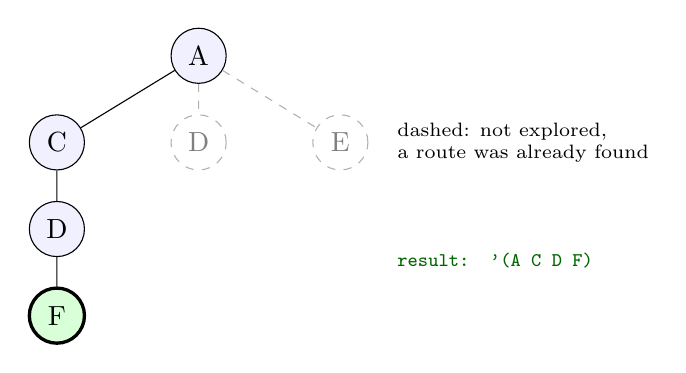
\begin{tikzpicture}[level distance=11mm,level 1/.style={sibling distance=18mm},
  v/.style={circle,draw,minimum size=7mm,fill=blue!6},
  u/.style={circle,draw=gray!60,dashed,minimum size=7mm,text=gray},
  g/.style={circle,draw,very thick,minimum size=7mm,fill=green!15}]
  \node[v] {A}
    child {node[v] {C} child {node[v] {D} child {node[g] {F}}}}
    child {node[u] {D} edge from parent[dashed,gray!60]}
    child {node[u] {E} edge from parent[dashed,gray!60]};
  \node[font=\scriptsize,align=left,anchor=west] at (2.4,-1.1) {dashed: not explored,\\a route was already found};
  \node[font=\scriptsize\ttfamily,anchor=west,green!40!black] at (2.4,-2.6) {result: '(A C D F)};
\end{tikzpicture}
\end{center}

\paragraph{Condensed trace.}
\begin{lstlisting}[style=racket]
(find-route 'A 'F g)
=> ... (find-route/list '(C D E) 'F g) ...
=> ... (find-route 'C 'F g) ...
=> ... (find-route/list '(D) 'F g) ...
=> ... (find-route 'D 'F g) ...
=> ... (find-route/list '(F) 'F g) ...
=> ... (find-route 'F 'F g) ...            ; produces '(F)
=> '(A C D F)                                ; conses back up the chain
\end{lstlisting}

\subsection{The problem with cycles}
If the graph has a cycle, say we add the edge $D \to A$, then searching from
\code{'A} for an unreachable node such as \code{'B} can go
$A \to C \to D \to A \to C \to \cdots$ forever. The functions above do not
terminate on cyclic graphs.

\begin{center}
\begin{tikzpicture}[->, >={Stealth}, node distance=16mm,
  every node/.style={circle,draw,minimum size=7mm}]
  \node (A) {A};
  \node (C) [right=of A] {C};
  \node (B) [below=of A] {B};
  \node (D) [below=of C] {D};
  \node (E) [right=of C] {E};
  \node (F) [right=of D] {F};
  \draw[very thick,red!70!black] (A) -- (C);
  \draw (A) -- (D); \draw (A) -- (E);
  \draw (B) -- (E); \draw (B) -- (F);
  \draw[very thick,red!70!black] (C) -- (D);
  \draw (D) -- (F);
  \draw (E) -- (F);
  \draw[very thick,red!70!black] (D) to[bend left=25] (A);
  \node[draw=none,font=\scriptsize,red!70!black,align=left,anchor=west] at ($(F.east)+(0.4,0.8)$) {new edge $D \to A$ closes\\the cycle $A \to C \to D \to A$};
\end{tikzpicture}
\end{center}

\subsection{Fix: an accumulator of visited nodes}
Keep a list of nodes already on the current path (or already visited) and
never revisit them.

\begin{lstlisting}[style=racket]
;; find-route: Node Node Graph -> (anyof (listof Node) false)
(define (find-route orig dest G)
  (find-route/acc orig dest G empty))

;; (find-route/acc orig dest G visited) finds a path from orig to dest
;;   that avoids the nodes in visited, or produces false.
;; find-route/acc: Node Node Graph (listof Node)
;;                 -> (anyof (listof Node) false)
(define (find-route/acc orig dest G visited)
  (cond [(symbol=? orig dest) (list orig)]
        [else (local [(define nbrs (neighbours orig G))
                      (define new-visited (cons orig visited))
                      (define route (find-route/list nbrs dest G new-visited))]
                (cond [(false? route) false]
                      [else (cons orig route)]))]))

;; find-route/list: (listof Node) Node Graph (listof Node)
;;                  -> (anyof (listof Node) false)
(define (find-route/list los dest G visited)
  (cond [(empty? los) false]
        [(member? (first los) visited)
         (find-route/list (rest los) dest G visited)]
        [else (local [(define route (find-route/acc (first los) dest G visited))]
                (cond [(false? route) (find-route/list (rest los) dest G visited)]
                      [else route]))]))
\end{lstlisting}

\begin{sloppypar}\noindent\textbf{Termination.} The measure is the number of graph nodes \emph{not} in
\code{visited}. Whenever \code{find-route/list} calls
\code{find-route/acc}, it does so on a node not in \code{visited}, and that node is added before the next
level, so the measure strictly decreases along every chain of calls.
\code{find-route/list} itself recurses structurally on \code{los}.
\end{sloppypar}

\paragraph{Efficiency.} With a visited list that only contains the current
path, the search can still revisit the same node through different paths,
which is exponential in the worst case. Passing back the set of
\emph{all} nodes explored so far (not just the current path) makes each node
expanded at most once; this is the idea behind depth-first search covered in
later courses (CS 341).

\section{Other graph problems}
\begin{itemize}
  \item \textbf{Reachability}: the set of nodes reachable from a given node.
  \item \textbf{Topological sort} of a DAG (e.g.\ ordering courses to respect prerequisites).
  \item \textbf{Shortest paths} (breadth-first search, Dijkstra's algorithm) --- later courses.
\end{itemize}

\section{Summary}
\begin{itemize}
  \item A directed graph is a set of vertices and directed edges; represented as an adjacency list.
  \item Path finding by backtracking: mutual recursion between a node function and a list-of-nodes function.
  \item On cyclic graphs, a visited accumulator is needed for termination.
  \item Termination measure: number of unvisited nodes.
\end{itemize}
